% ==============================================================================
% Modelo para Especificação de Projeto de Software
% Prof. Vítor E. Silva Souza - NEMO/UFES :: DI/UFES :: PPGI/UFES
%
% Baseado em abtex2-modelo-trabalho-academico.tex, v-1.9.2 laurocesar
% Copyright 2012-2014 by abnTeX2 group at http://abntex2.googlecode.com/ 
%
% This work may be distributed and/or modified under the conditions of the LaTeX 
% Project Public License, either version 1.3 of this license or (at your option) 
% any later version. The latest version of this license is in
% http://www.latex-project.org/lppl.txt.
%
% IMPORTANTE:
% Instruções encontram-se espalhadas pelo documento. Para facilitar sua leitura,
% tais instruções são precedidas por (*) -- utilize a função localizar do seu
% editor para passar por todas elas.
% ==============================================================================

% Usa o estilo abntex2, configurando detalhes de formatação e hifenização.
\documentclass[
	12pt,				
	oneside,		
	a4paper,			
	english,			% Idioma adicional para hifenização.
	french,				% Idioma adicional para hifenização.
	spanish,			% Idioma adicional para hifenização.
	brazil				% O último idioma é o principal do documento.
	]{abntex2}


%%% Importação de pacotes. %%%

% Conserta o erro "No room for a new \count". 
% O comando \reserveinserts deve ser comentado ou não, dependendo da versão do LaTeX.
\usepackage{etex}
%\reserveinserts{28}

% Usa a fonte Latin Modern.
\usepackage{lmodern}

% Seleção de códigos de fonte.
\usepackage[T1]{fontenc}

% Codificação do documento em Unicode.
\usepackage[utf8]{inputenc}

% Usado pela ficha catalográfica.
\usepackage{lastpage}

% Indenta o primeiro parágrafo de cada seção.
\usepackage{indentfirst}

% Controle das cores.
\usepackage[usenames,dvipsnames]{xcolor}

% Inclusão de gráficos.
\usepackage{graphicx}

% Melhor controle de leiaute de tabelas.
\usepackage{tabularx}
\usepackage{colortbl}
\usepackage{longtable}
\usepackage{pdflscape}

% Inclusão de páginas em PDF diretamente no documento (para uso nos apêndices).
\usepackage{pdfpages}

\usepackage{float}


% Para melhorias de justificação.
\usepackage{microtype}

% Citações padrão ABNT.
\usepackage[brazilian,hyperpageref]{backref}
\usepackage[alf]{abntex2cite}	
\renewcommand{\backrefpagesname}{Citado na(s) página(s):~}		% Usado sem a opção hyperpageref de backref.
\renewcommand{\backref}{}										% Texto padrão antes do número das páginas.
\renewcommand*{\backrefalt}[4]{									% Define os textos da citação.
	\ifcase #1
		Nenhuma citação no texto.
	\or
		Citado na página #2.
	\else
		Citado #1 vezes nas páginas #2.
	\fi}

% \rm is deprecated and should not be used in a LaTeX2e document
% http://tex.stackexchange.com/questions/151897/always-textrm-never-rm-a-counterexample
\renewcommand{\rm}{\textrm}

% Inclusão de símbolos não padrão.
\usepackage{amssymb}
\usepackage{eurosym}

% Para utilizar \eqref para referenciar equações.
\usepackage{amsmath}

% Permite mostrar figuras muito largas em modo paisagem com \begin{sidewaysfigure} ao invés de \begin{figure}.
\usepackage{rotating}

% Permite customizar listas enumeradas/com marcadores.
\usepackage{enumitem}

% Permite inserir hiperlinks com \url{}.
\usepackage{bigfoot}
\usepackage{hyperref}

% Permite usar o comando \hl{} para evidenciar texto com fundo amarelo. Útil para chamar atenção a itens a fazer.
\usepackage{soulutf8}

% Colorinlistoftodos package: to insert colored comments so authors can collaborate on the content.
% (*) Indicar o nome do aluno e substituir o nome do professor se for o caso.
\usepackage[colorinlistoftodos, textwidth=20mm, textsize=footnotesize]{todonotes}
\newcommand{\aluno}[1]{\todo[author=\textbf{Aluno},color=green!30,caption={},inline]{#1}}
\newcommand{\vitor}[1]{\todo[author=\textbf{Vítor},color=red!30,caption={},inline]{#1}}

% Permite inserir espaço em branco condicional (incluído no texto final só se necessário) em macros.
\usepackage{xspace}

% Permite incluir listagens de código com o comando \lstinputlisting{}.
\usepackage{listings}
\usepackage{caption}
\DeclareCaptionFont{white}{\color{white}}
\DeclareCaptionFormat{listing}{\colorbox{gray}{\parbox{\textwidth}{#1#2#3}}}
\captionsetup[lstlisting]{format=listing,labelfont=white,textfont=white}
\renewcommand{\lstlistingname}{Listagem}
\definecolor{mygray}{rgb}{0.5,0.5,0.5}
\lstset{
	basicstyle=\scriptsize,
	breaklines=true,
	numbers=left,
	numbersep=5pt,
	numberstyle=\tiny\color{mygray}, 
	rulecolor=\color{black},
	showstringspaces=false,
	tabsize=2,
    inputencoding=utf8,
    extendedchars=true,
    literate=%
    {é}{{\'{e}}}1
    {è}{{\`{e}}}1
    {ê}{{\^{e}}}1
    {ë}{{\¨{e}}}1
    {É}{{\'{E}}}1
    {Ê}{{\^{E}}}1
    {û}{{\^{u}}}1
    {ù}{{\`{u}}}1
    {â}{{\^{a}}}1
    {à}{{\`{a}}}1
    {á}{{\'{a}}}1
    {ã}{{\~{a}}}1
    {Á}{{\'{A}}}1
    {Â}{{\^{A}}}1
    {Ã}{{\~{A}}}1
    {ç}{{\c{c}}}1
    {Ç}{{\c{C}}}1
    {õ}{{\~{o}}}1
    {ó}{{\'{o}}}1
    {ô}{{\^{o}}}1
    {Õ}{{\~{O}}}1
    {Ó}{{\'{O}}}1
    {Ô}{{\^{O}}}1
    {î}{{\^{i}}}1
    {Î}{{\^{I}}}1
    {í}{{\'{i}}}1
    {Í}{{\~{Í}}}1
}




%%% Definição de variáveis. %%%
% (*) Substituir os textos abaixo com as informações apropriadas.
\titulo{Site do ConneCT}
\autor{Nome do Aluno}
\local{Vitória, ES}
\data{\the\year}
\instituicao{
	Universidade Federal do Espírito Santo -- UFES
	\par
	Centro Tecnológico
	\par
	Departamento de Informática}
\newcommand{\subtitulo}{Documento de Projeto de Sistema}
\newcommand{\versao}{1.0}

% Define a capa.
\renewcommand{\imprimircapa}{%
	\begin{capa}%
		\center
		
		{\ABNTEXchapterfont\large\subtitulo{}}
		\vfill
		\begin{center}
			\ABNTEXchapterfont\bfseries\LARGE\imprimirtitulo
		\end{center}
		
		\vfill
		\large\imprimirlocal
		\linebreak
		\large\imprimirdata
		\vspace*{1cm}
	\end{capa}
}

% Macros específicas do trabalho.
% (*) Inclua aqui termos que são utilizados muitas vezes e que demandam formatação especial.
% Exemplo: Java com TM (trademark) em superscript.
% Use sempre \xspace para que o LaTeX inclua espaço em branco após a macro somente quando necessário.
\newcommand{\java}{Java\texttrademark\xspace}




%%% Configurações finais de aparência. %%%

% Altera o aspecto de algumas cores.
\definecolor{blue}{RGB}{41,5,195}
\definecolor{lightgray}{gray}{0.9}

% Informações do PDF.
\makeatletter
\hypersetup{
	pdftitle={\@title}, 
	pdfauthor={\@author},
	pdfsubject={\imprimirpreambulo},
	pdfcreator={LaTeX with abnTeX2},
	pdfkeywords={abnt}{latex}{abntex}{abntex2}{trabalho acadêmico}, 
	colorlinks=true,				% Colore os links (ao invés de usar caixas).
	linkcolor=blue,					% Cor dos links.
	citecolor=blue,					% Cor dos links na bibliografia.
	filecolor=magenta,				% Cor dos links de arquivo.
	urlcolor=blue,					% Cor das URLs.
	bookmarksdepth=4
}
\makeatother

% Espaçamentos entre linhas e parágrafos.
\setlength{\parindent}{1.3cm}
\setlength{\parskip}{0.2cm}



%%% Páginas iniciais do documento: capa, folha de rosto, ficha, resumo, tabelas, etc. %%%

% Compila o índice.
\makeindex

% Inicia o documento.
\begin{document}

% Retira espaço extra obsoleto entre as frases.
\frenchspacing

% Inclui o brasão da UFES.
\begin{figure}[h]
  \centering
  
\includegraphics[scale=0.055]{brasao.jpg}
  \label{ppts3}
\end{figure} 

% Capa do trabalho.
\imprimircapa


% (*) Incluir linhas no registro de alterações a cada nova versão.
\begin{center}
	{\large\bfseries Registro de Alterações:}
	
	\vspace{0.5cm}
	\begin{tabular}{|c|p{45mm}|c|p{60mm}|} \hline
		
		\textbf{Versão} & \textbf{Responsável} & \textbf{Data}  & \textbf{Alterações} \\ \hline   
		
		1.0  & Guilherme & 25/05/2025 & Versão inicial. \\\hline 
	\end{tabular}
\end{center}
\newpage



%%% Início da parte de conteúdo do documento. %%%
% Marca o início dos elementos textuais.
\textual

\begingroup
\let\clearpage\relax

% ==============================================================================
% Projeto de Sistema - Nome do Aluno
% Capítulo 1 - Introdução
% ==============================================================================
\chapter{Introdução}
\label{sec-intro}
\vspace{-1cm}

Este documento apresenta o projeto (\textit{design}) do sistema \emph{\imprimirtitulo}. O ConneCT é um projeto de extensão da UFES e seu site deve oferecer opções de cadastro de alunos  e professores que participam do projeto, além de divulgar informações relevantes sobre o projeto e possibilitar interação com coordenadores do mesmo.


Além desta introdução, este documento está organizado da seguinte forma: 
a Seção~\ref{sec-plataforma} apresenta a plataforma de software utilizada na implementação do sistema; 
a Seção~\ref{sec-arquitetura} apresenta a arquitetura de software; por fim, 
a Seção~\ref{sec-frameweb} apresenta os modelos FrameWeb que descrevem os componentes da arquitetura.


\vspace*{1cm}

% ==============================================================================
% Projeto de Sistema - Nome do Aluno
% Capítulo 2 - Plataforma de Desenvolvimento
% ==============================================================================
\chapter{Plataforma de Desenvolvimento}
\label{sec-plataforma}
\vspace{-1cm}


%=======================================================================================================
%			Tabela de Plataforma de Desenvolvimento e Tecnologias Utilizadas
%=======================================================================================================

Na Tabela~\ref{tabela-plataforma} são listadas as tecnologias utilizadas no desenvolvimento da ferramenta, bem como o propósito de sua utilização.

\begin{footnotesize}
\begin{longtable}{|p{1.8cm}|c|p{5cm}|p{6.3cm}|}
	\caption{Plataforma de Desenvolvimento e Tecnologias Utilizadas.}	
	\label{tabela-plataforma}\\\hline

	\rowcolor{lightgray}
	\textbf{Tecnologia} & \textbf{Versão} & \textbf{Descrição} & \textbf{Propósito} \\\hline 
	\endfirsthead
	\hline
	\rowcolor{lightgray}
	\textbf{Tecnologia} & \textbf{Versão} & \textbf{Descrição} & \textbf{Propósito} \\\hline 
	\endhead	

	Python & 3.12 & Linguagem de programação de alto nível, orientada a objetos, com tipagem dinâmica. & Escrita do código-fonte das classes que compõem o sistema. \\\hline
	
	Flask & 3.0 & Microframework para construção de aplicações Web. & Desenvolvimento de APIs RESTful e aplicações Web com arquitetura leve e extensível.  \\\hline  
	
	Jinja2 & 3.1 & 	Motor de templates integrado ao Flask. & Definição de templates HTML, promovendo a separação entre lógica de negócio e camada de apresentação. \\\hline
	
	SQLAlchemy & 2.0 & ORM (Object Relational Mapper) para persistência de dados em bancos relacionais. & Persistência dos objetos de domínio sem necessidade de escrita direta de comandos SQL. \\\hline
	
	Marshmallow & 3.20 & Biblioteca para serialização e validação de objetos. & Facilita a validação e transformação de objetos Python em formatos como JSON, e vice-versa. \\\hline
	
	Alembic & 1.12 &  Ferramenta de migração de banco de dados. & Controle e versionamento do esquema do banco de dados. \\\hline
	
	Gunicorn & 21.2 &  Servidor WSGI para aplicações Python. & Hospedagem e execução da aplicação Web, intermediando requisições HTTP e a aplicação Flask. \\\hline
	
	MySQL Server & 8.0 & Sistema Gerenciador de Banco de Dados Relacional gratuito. & Armazenamento dos dados manipulados pela ferramenta. \\\hline
	
	Docker & 26.0 & Plataforma para criação, execução e gerenciamento de containers. & Facilita o empacotamento e a distribuição do ambiente de desenvolvimento e produção da aplicação. \\\hline
\end{longtable}
\end{footnotesize}






%=======================================================================================================
%			Tabela de Softwares de Apoio ao Desenvolvimento do Projeto
%=======================================================================================================

Na Tabela~\ref{tabela-software} vemos os softwares que apoiaram o desenvolvimento de documentos e também do código fonte.

\begin{footnotesize}
\begin{longtable}{|p{2.5cm}|c|p{5cm}|p{5.5cm}|}
	\caption{Softwares de Apoio ao Desenvolvimento do Projeto}	
	\label{tabela-software}\\\hline
	
	\rowcolor{lightgray}
	\textbf{Tecnologia} & \textbf{Versão} & \textbf{Descrição} & \textbf{Propósito} \\\hline 
	\endfirsthead
	\hline
	\rowcolor{lightgray}
	\textbf{Tecnologia} & \textbf{Versão} & \textbf{Descrição} & \textbf{Propósito} \\\hline 
	\endhead
	 
	FrameWeb Plugin for Visual Paradigm & 1.0 & Extensão do Visual Paradigm que implementa o método FrameWeb. & Apoio na modelagem arquitetural e geração de artefatos conforme o método FrameWeb. \\\hline

	Overleaf  & 5.4.1 & Editor online colaborativo de LaTeX. & Escrita colaborativa da documentação do sistema, utilizando o template abnTeX. \\\hline        

	Visual Paradigm & 17.3 & Editor UML com suporte ao método FrameWeb via plug-in. & Criação dos modelos de Entidades, Aplicação, Persistência e Navegação conforme o método FrameWeb. \\\hline 
	
	Apache Maven & 3.5 & Ferramenta de gerência/construção de projetos de software. & Obtenção e integração das dependências do projeto. \\\hline
\end{longtable}
\end{footnotesize}

\vspace*{1cm}

\endgroup


\chapter{Arquitetura de Software}
\label{sec-arquitetura}
\vspace{-1cm}

A Figura~\ref{figura-arquitetura} mostra a arquitetura do sistema \emph{\imprimirtitulo}.

\begin{figure}[h]
	\centering
	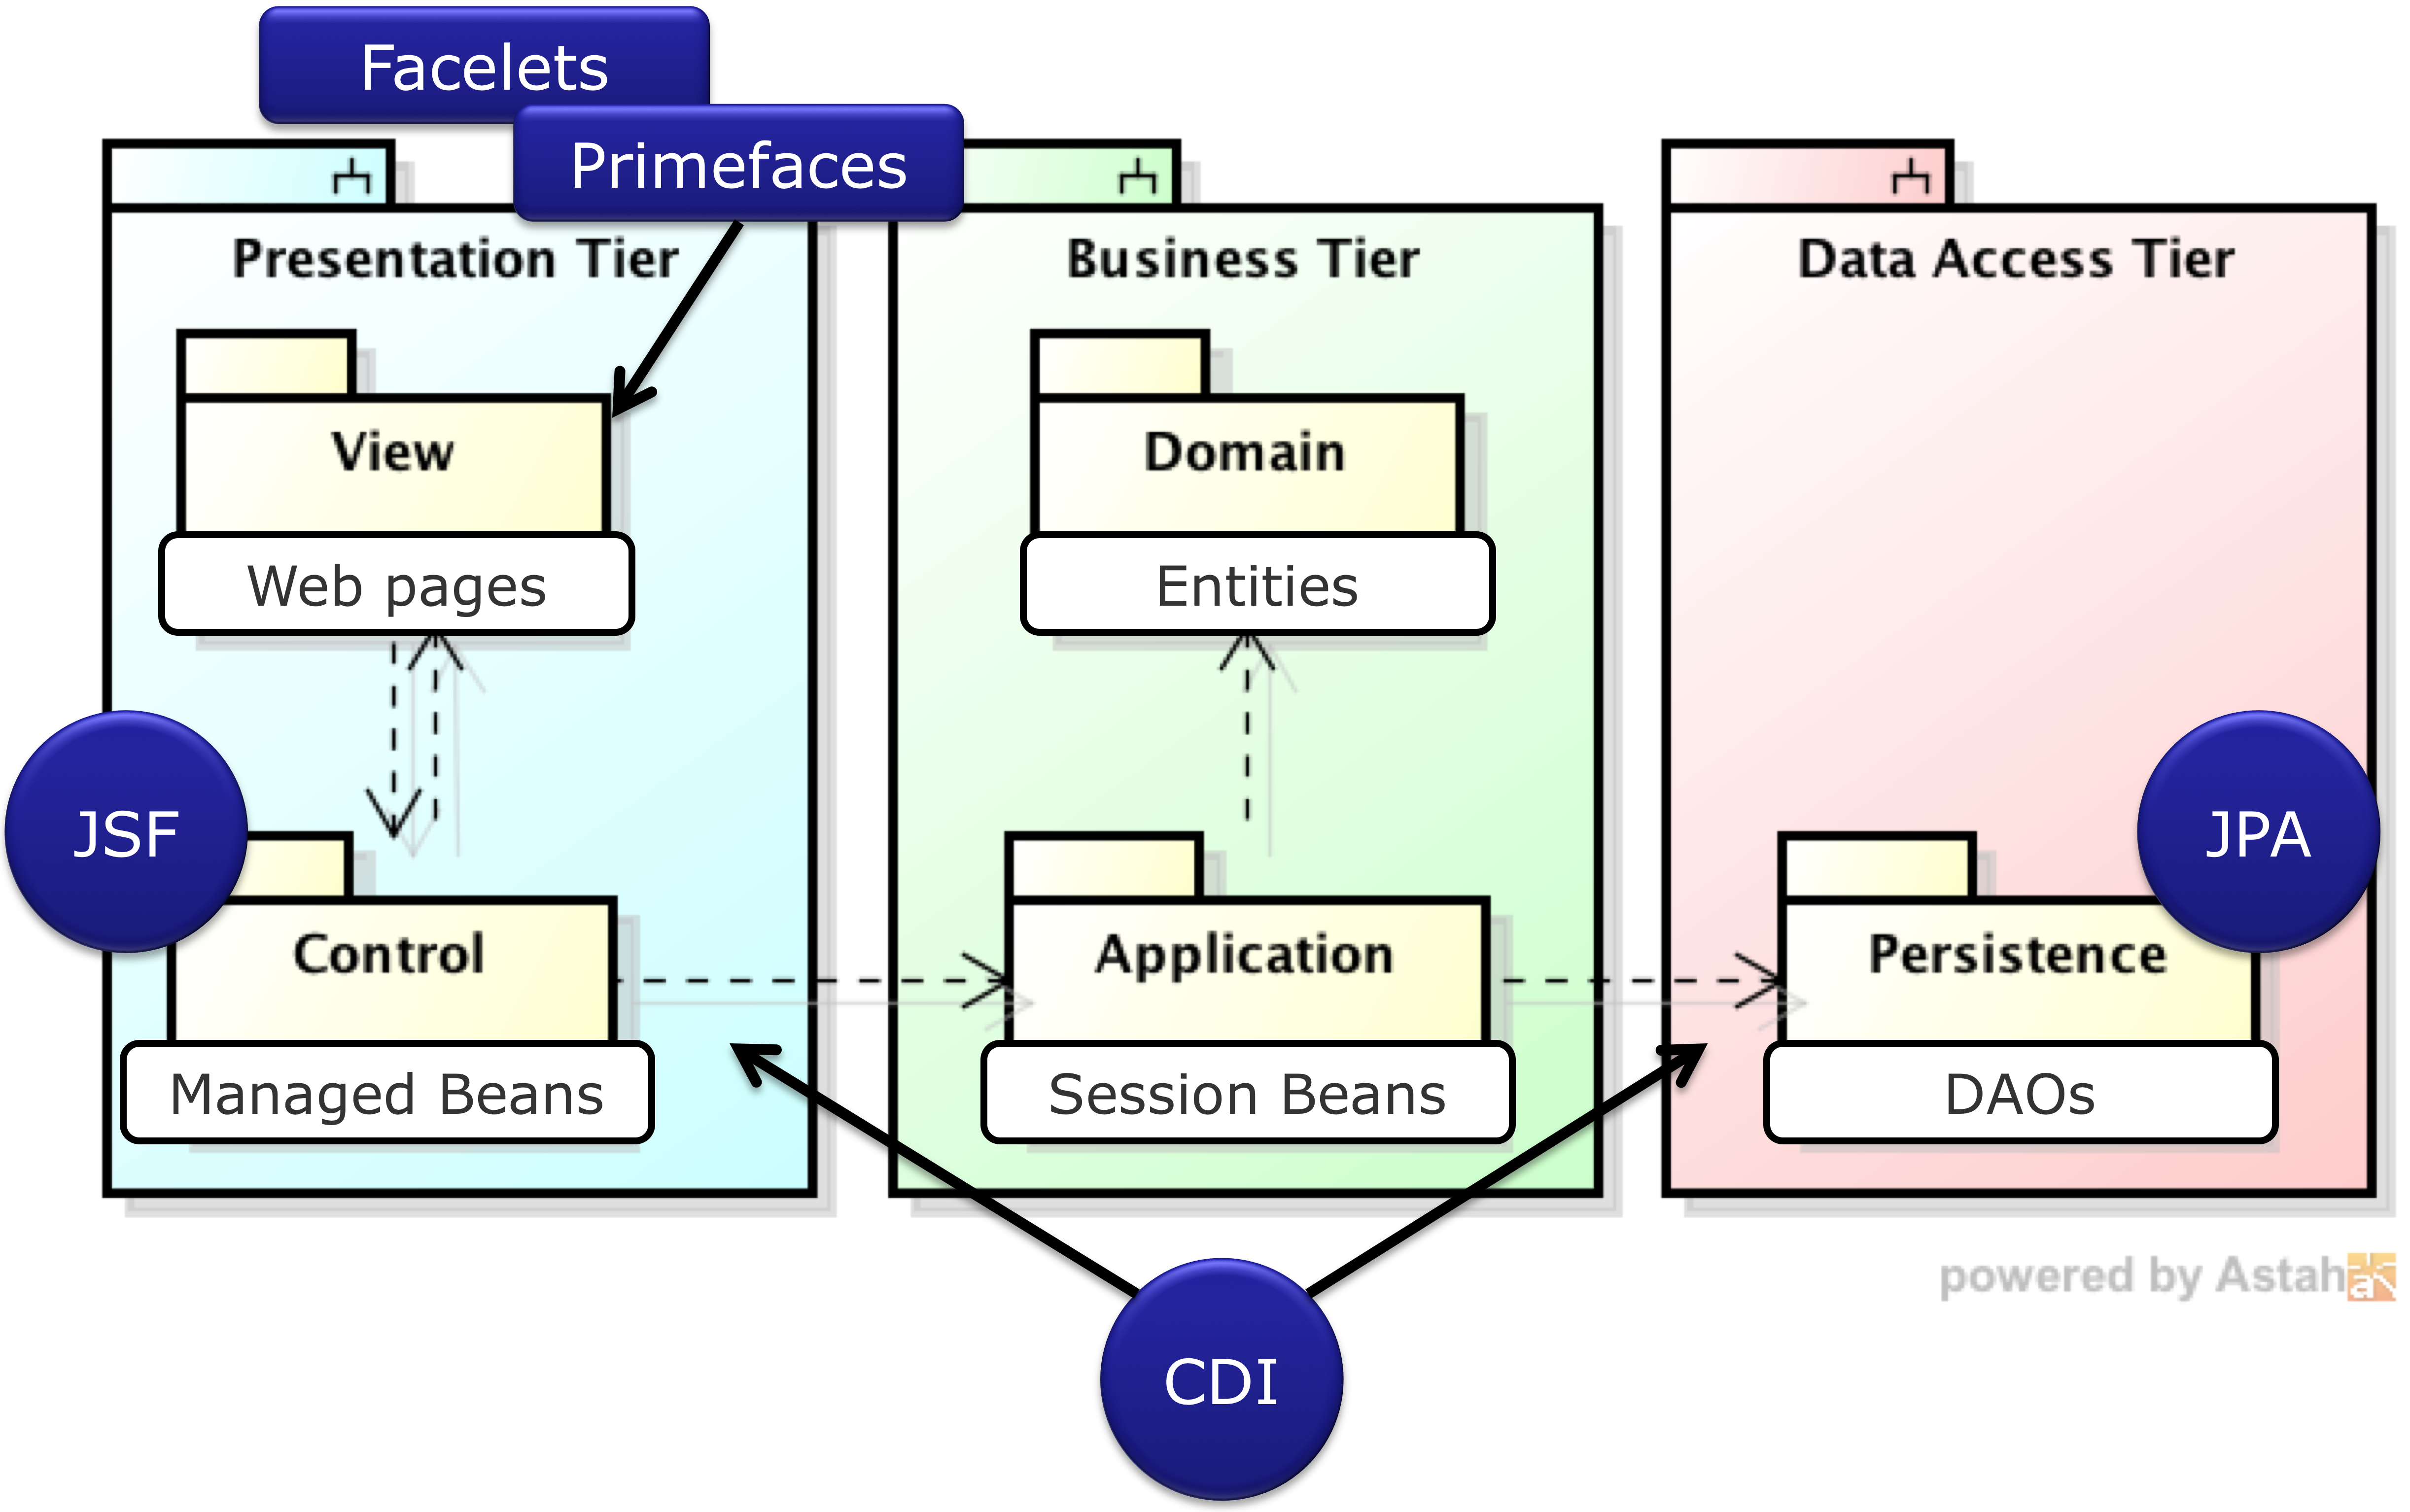
\includegraphics[width=0.8\textwidth]{figuras/figura-arquitetura-padrao.png}
	\caption{Arquitetura de Software.}
	\label{figura-arquitetura}
\end{figure}



\chapter{Modelagem FrameWeb}
\label{sec-frameweb}
\vspace{-1cm}

\emph{\imprimirtitulo} é um sistema Web cuja arquitetura utiliza \textit{frameworks} comuns no desenvolvimento para esta plataforma. Desta forma, o sistema pode ser modelado utilizando a abordagem FrameWeb~\cite{souza-celebratingfalbo20}.

A Tabela~\ref{tabela-frameworks} indica os \textit{frameworks} presentes na arquitetura do sistema que se encaixam em cada uma das categorias de \textit{frameworks} que FrameWeb dá suporte. Em seguida, os modelos FrameWeb são apresentados para cada camada da arquitetura.

\begin{footnotesize}
	\begin{longtable}{|c|c|}
		\caption{\textit{Frameworks} da arquitetura do sistema separados por categoria.}
		\label{tabela-frameworks}\\\hline
		
		\rowcolor{lightgray}
		\textbf{Categoria de \textit{Framework}} & \textbf{\textit{Framework} Utilizado} \\\hline 
		\endfirsthead
		\hline
		\rowcolor{lightgray}
		\textbf{Categoria de \textit{Framework}} & \textbf{\textit{Framework} Utilizado} \\\hline 
		\endhead

		Controlador Frontal & Flask \\\hline

		Injeção de Dependências & Flask (Blueprints e extensões) \\\hline

		Mapeamento Objeto/Relacional & SQLAlchemy \\\hline

		Segurança & Flask Security \\\hline
	\end{longtable}
\end{footnotesize}

\section{Camada de Negócio}
\label{sec-frameweb-negocio}

\begin{figure}[H]
	\centering
	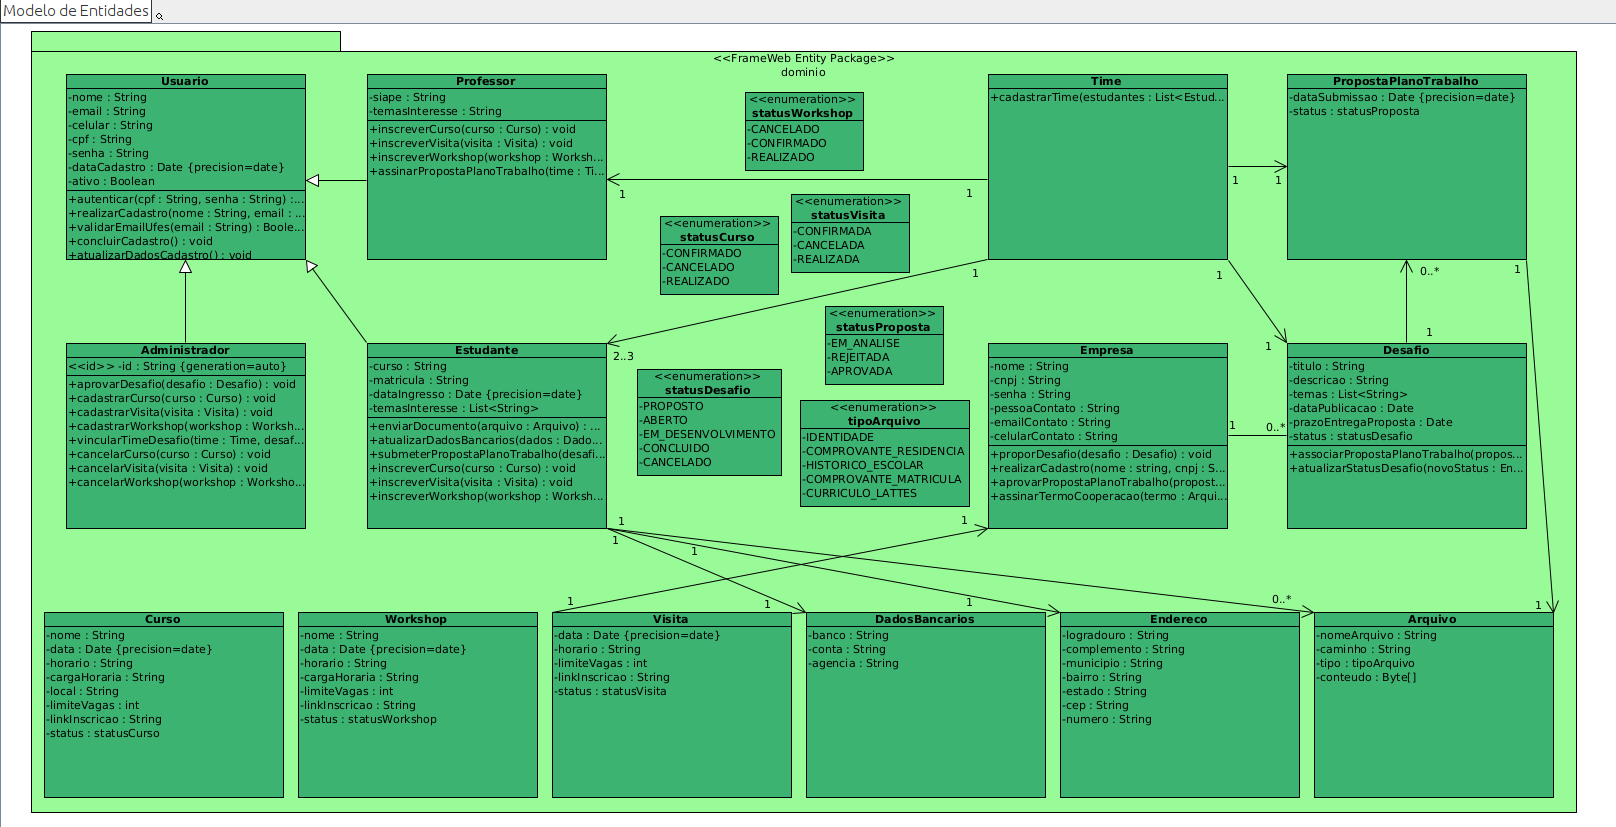
\includegraphics[width=1.0\textwidth]{figuras/figura_modelo_entidades.png}
	\caption{Modelo de entidades do FrameWeb.}
	\label{figura-entidades}
\end{figure}

\begin{figure}[H]
	\centering
	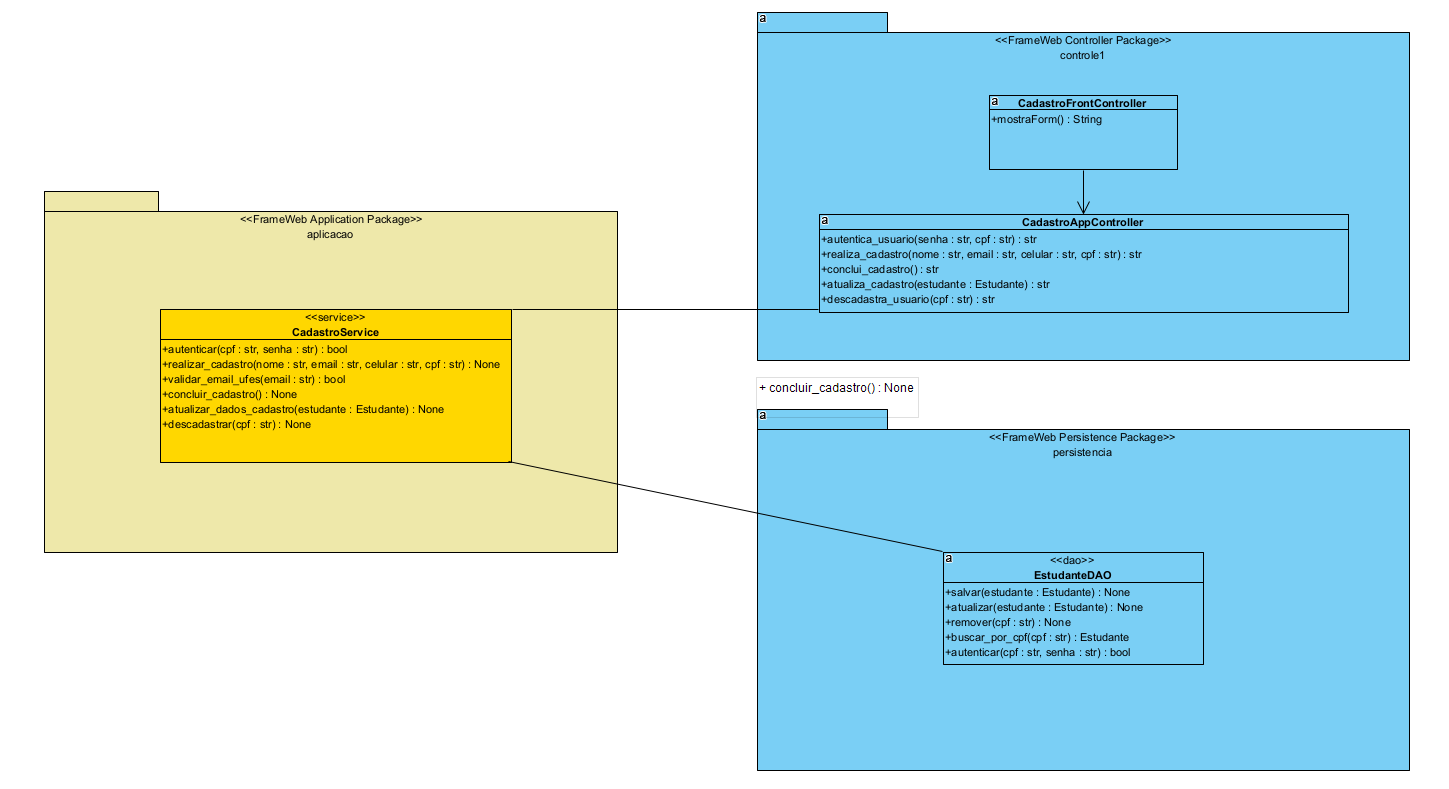
\includegraphics[width=1.0\textwidth]{figuras/figura_modelo_aplicacao.png}
	\caption{Modelo de aplicação do FrameWeb: Cadastro de Estudantes.}
	\label{figura-aplicacao}
\end{figure}

\section{Camada de Acesso a Dados}
\label{sec-frameweb-dados}

\begin{figure}[H]
	\centering
	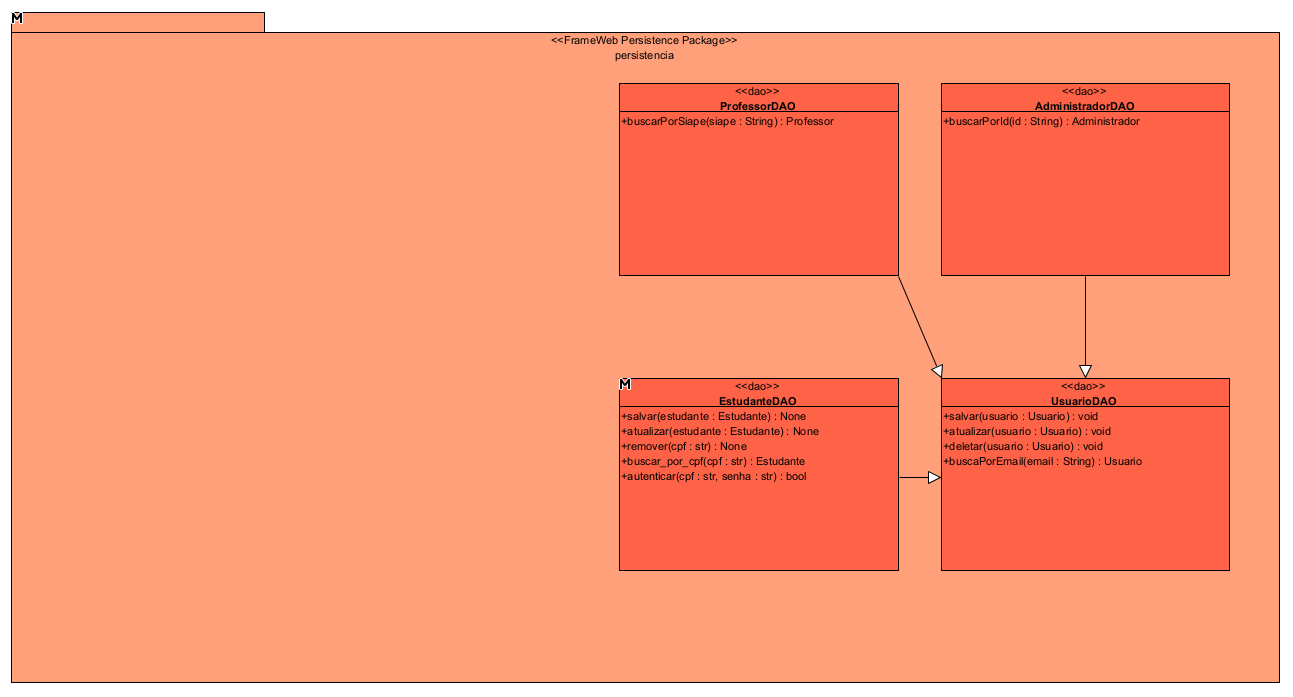
\includegraphics[width=1.0\textwidth]{figuras/figura_modelo_persistencia.png}
	\caption{Modelo de persistência do FrameWeb: Usuário.}
	\label{figura-persistencia}
\end{figure}

\section{Camada de Apresentação}
\label{sec-frameweb-apresentacao}

\begin{figure}[H]
	\centering
	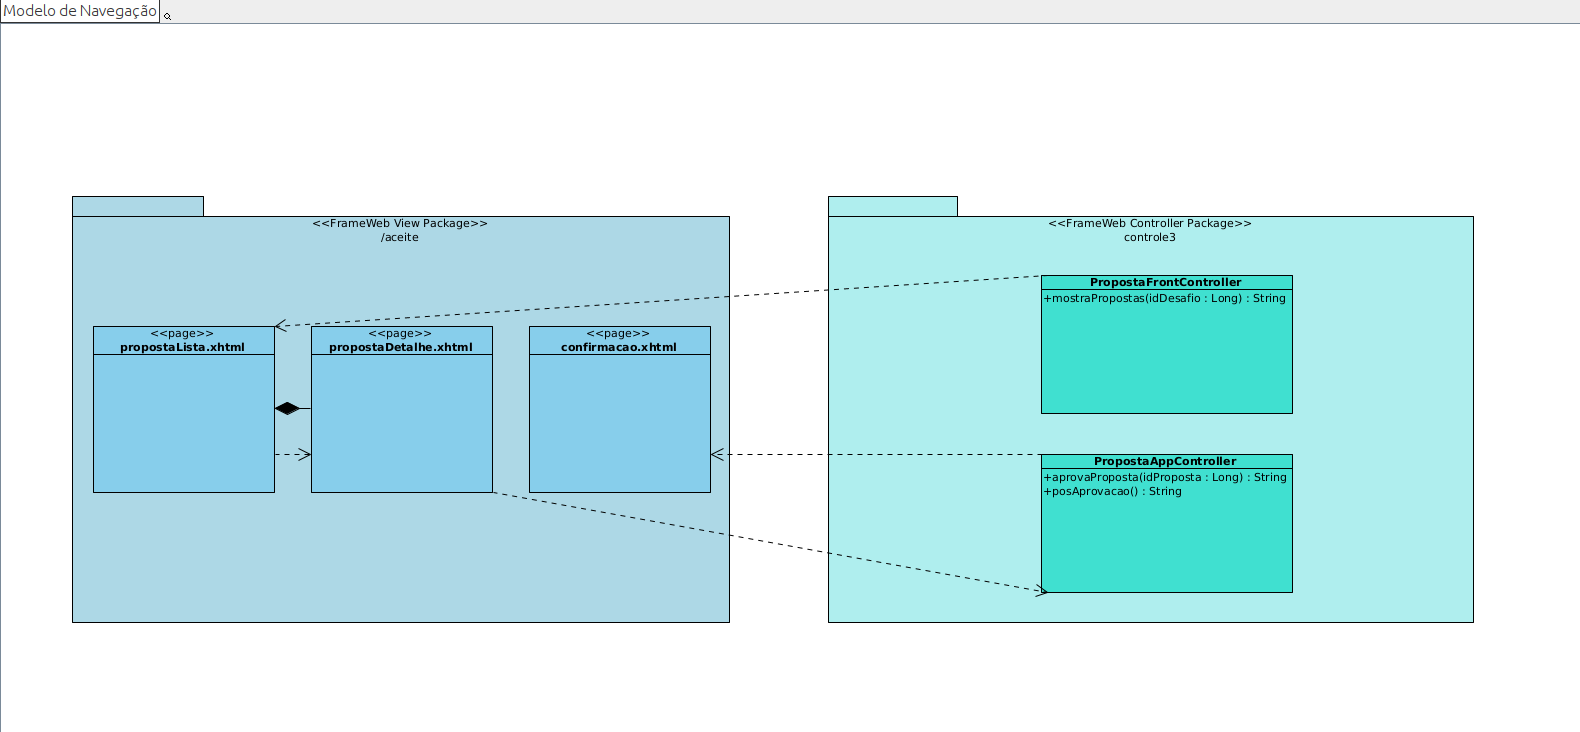
\includegraphics[width=1.0\textwidth]{figuras/figura_modelo_navegacao_cadastro.png}
	\caption{Modelo de navegação do FrameWeb - Cadastro.}
	\label{figura-cadastro}
\end{figure}

\begin{figure}[H]
	\centering
	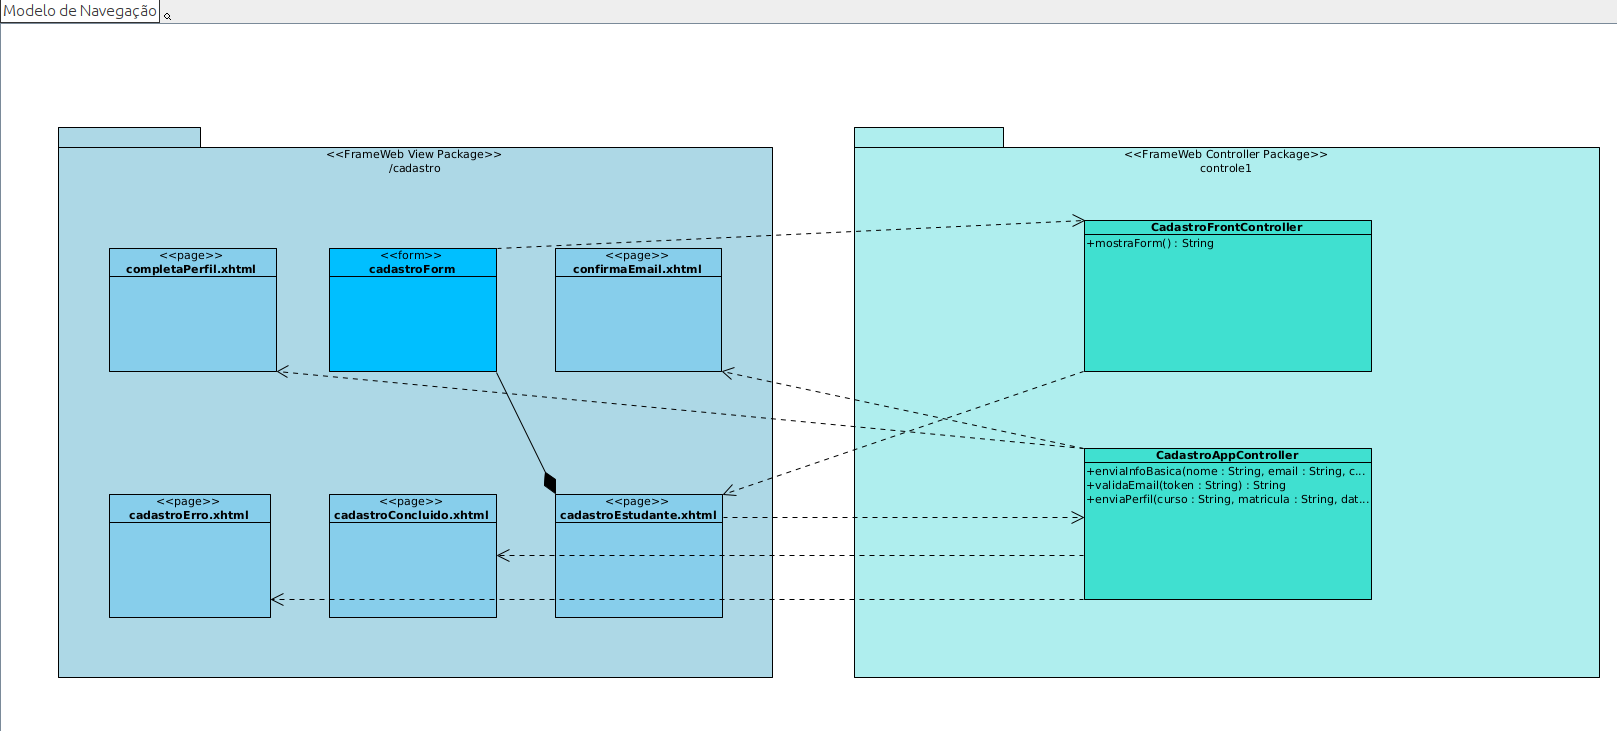
\includegraphics[width=1.0\textwidth]{figuras/figura_modelo_navegacao_notificacao.png}
	\caption{Modelo de navegação do FrameWeb - Notificação.}
	\label{figura-notificacao}
\end{figure}

\begin{figure}[H]
	\centering
	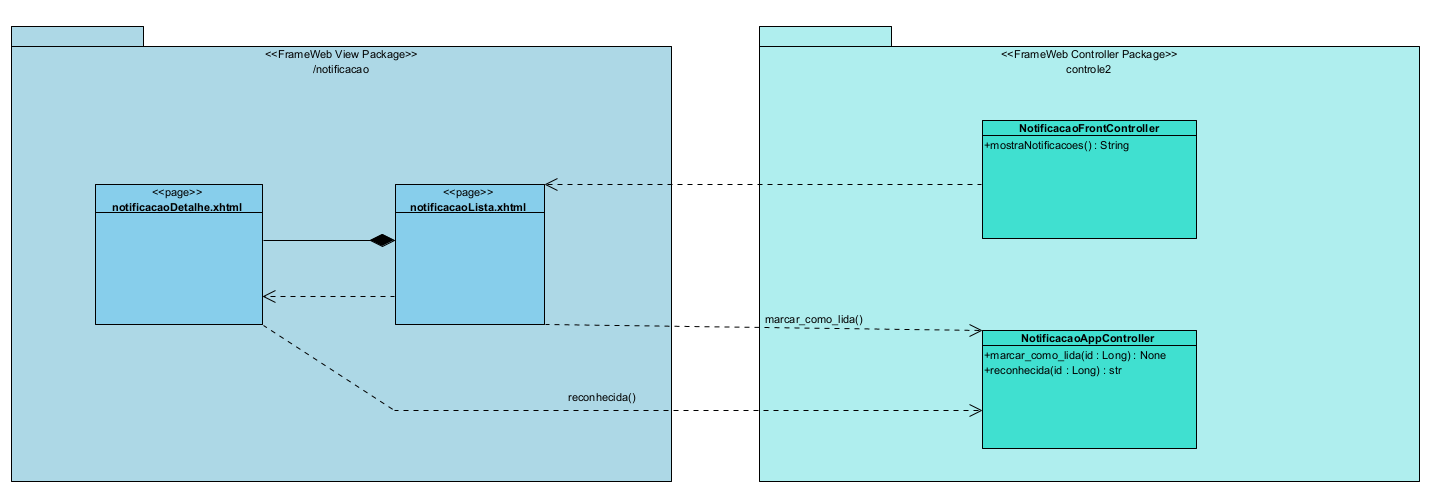
\includegraphics[width=1.0\textwidth]{figuras/figura_modelo_navegacao_aceite.png}
	\caption{Modelo de navegação do FrameWeb - Aceite.}
	\label{figura-aceite}
\end{figure}








%%% Páginas finais do documento: bibliografia e anexos. %%%
% Finaliza a parte no bookmark do PDF para que se inicie o bookmark na raiz e adiciona espaço de parte no sumário.
\phantompart

% Marca o início dos elementos pós-textuais.
\postextual

% Referências bibliográficas
\bibliography{bibliografia}

% Índice remissivo.
\phantompart
\printindex

% Fim do documento.
\end{document}
